\documentclass[a4paper,10pt]{article}
\usepackage{listings}
\usepackage{graphicx}
\title{\vspace{-1.5em}\textbf{ID1206 Operating Systems}}
\author{{\textbf{Isak Nyberg}} \\
        {\textbf{Seminar 3 Green Threads}}
        }


\newcommand{\code}[1]{\texttt{#1}}


\usepackage{color}
\definecolor{mygreen}{rgb}{0,0.6,0}
\definecolor{mygray}{rgb}{0.5,0.5,0.5}
\definecolor{mymauve}{rgb}{0.58,0,0.82}

\lstset{ 
  backgroundcolor=\color{white},   % choose the background color; you must add \usepackage{color} or \usepackage{xcolor}; should come as last argument
  basicstyle=\footnotesize,        % the size of the fonts that are used for the code
  breakatwhitespace=true,          % sets if automatic breaks should only happen at whitespace
  breaklines=true,                 % sets automatic line breaking
  captionpos=b,                    % sets the caption-position to bottom
  commentstyle=\color{mygreen},    % comment style
  deletekeywords={...},            % if you want to delete keywords from the given language
  escapeinside={\%*}{*)},          % if you want to add LaTeX within your code
  extendedchars=true,              % lets you use non-ASCII characters; for 8-bits encodings only, does not work with UTF-8
  firstnumber=1,                   % start line enumeration with line 1000
  frame=single,                    % adds a frame around the code
  keepspaces=true,                 % keeps spaces in text, useful for keeping indentation of code (possibly needs columns=flexible)
  keywordstyle=\color{blue},       % keyword style
  language=C,                      % the language of the code
  morekeywords={*,...},            % if you want to add more keywords to the set
  numbers=left,                    % where to put the line-numbers; possible values are (none, left, right)
  numbersep=5pt,                   % how far the line-numbers are from the code
  numberstyle=\tiny\color{mygray}, % the style that is used for the line-numbers
  rulecolor=\color{black},         % if not set, the frame-color may be changed on line-breaks within not-black text (e.g. comments (green here))
  showspaces=false,                % show spaces everywhere adding particular underscores; it overrides 'showstringspaces'
  showstringspaces=false,          % underline spaces within strings only
  showtabs=false,                  % show tabs within strings adding particular underscores
  stepnumber=1,                    % the step between two line-numbers. If it's 1, each line will be numbered
  stringstyle=\color{mymauve},     % string literal style
  tabsize=2,                       % sets default tabsize to 2 spaces
  inputencoding=utf8,
  literate={å}{{\'a}}1 {ä}{{\"a}}1 {Ä}{{\"A}}1 {ö}{{\"o}}1,
  title=\lstname                   % show the filename of files included with \lstinputlisting; also try caption instead of title
}

\begin{document}
\maketitle

\section*{Introduction}
When a process needs to have separate contexts to work on a task, it may need to make use of threads. A common example of this is a webpage server that needs to serve an incoming request while also listening for new request. In this case a thread would be created for every incoming request. In C this is implemented using the library pthreads which includes the functions \emph{green\_create()}, \emph{green\_yield()}, and \emph{green\_join()}. These all serve different functions when combined with the \emph{pthread\_t} struct. These threads however run in kernel space as the scheduling of the threads use the same scheduler as the operating system. A different way of implementing this is so called \emph{green threads}, these threads are instead managed in user space. This can be done using the \emph{make\_context()}, \emph{set\_context()}, \emph{swap\_context()} functions, which allow user-level context switching between multiple threads.

\section*{Thread and Ready queue}
A basic implementation of a thread would consist of its context, its instructions in the from of a function. However in order to interact with other threads the implementation needs to be extended further.

\begin{lstlisting}[title=Thread structure]
typedef struct green_t {
    ucontext_t *context;    // The stack and stack pointer
    void *(*fun)(void*);    // The function to execute
    void *arg;              // The arguments for the function
    struct green_t *next;   // Used for the different thread queues
    struct green_t *join;   // Pointer to joining threads
    void *retval;           // Where to store the return value
    int zombie;             // If true the process has terminated
} green_t;
\end{lstlisting}
Now a ready-queue can be created as a pointer to a thread that is not running and the next pointer will point to next thread in the queue. Now a running thread will run until it calls the function \emph{green\_yield()}, then the thread will add itself to the end of the ready-queue and switch context and begin execution of the first thread in the ready-queue until this thread in turn calls \emph{green\_yield()}.
\newpage
\section*{Joining}
When a thread needs to wait for another thread to terminate execution and collect its result it uses the \emph{green\_join()} function. This function needs a target thread and a pointer to where the thread should store its return value. What this will do is to first check if target thread has finished execution by checking the \emph{green->zombie} property. If the thread is still running, it will add itself to to the join pointer of the target thread so that the target thread knows it is being waited for. Thereafter the currently running thread will switch context to the next thread in the ready-queue without adding itself to the queue, effectively suspending itself until the thread it is waiting for has finished execution. When the target thread eventually terminates the result will be collected and its context will be freed from the heap. 

\begin{lstlisting}[title=Thread Joining]
int green_join(green_t *thread, void **res) {
    if (thread->zombie == FALSE){   // has target terminated?
        green_t *susp = running;
        thread->join = susp;    // tell target its being waited for
        green_t *next = ready_queu_pop();   // find next thread
        running = next;
        swapcontext(susp->context, next->context); // schedule next
    }
    // target thread has terminated
    if (thread->retval != NULL) {  // collect result
        res = thread->retval;
    }
    free(thread->context->uc_stack.ss_sp);  // free context of 
    free(thread->context);                  // terminated thread
    return 0;
}
\end{lstlisting}
With all of this implemented thread can now execute on their own, yield to each other and then wait for another thread to terminate and collect the result. However once the threads work together and make changes to shared data structures and variables further implementations is needed to ensure concurrency.


\section*{Conditional Suspending}
An added functionality for a thread is to voluntarily suspend and only wake up once another thread tells it to. In the pthread library this functionality is added with the \emph{pthread\_cond\_t}. This is a structure that combined with \emph{pthread\_cond\_wait()} and \emph{pthread\_cond\_signal()}. What wait will do is simply suspend the thread that called it without adding back it to the ready-queue, effectively making sure it will not run again until another thread calls signal on the same \emph{pthread\_cond\_t} variable. When signal is called the thread that has waited the longest for the condition is added back to the ready queue. This can lead to unintended consequences where some threads are sleeping forever if they are not woken up by another thread, however this is a problem the end user of the library has to take care of.
\newpage
\section*{Timer and Mutual Exclusion}
Instead of only suspend on conditions or when yielding, pthreads also suspends periodically when a thread has been running for a while. This is done with a timer interrupt and the suspended thread is added to the back of the ready-queue and the first thread in the ready-queue takes over execution. However this runs into some issue when a thread is interrupted in the middle of an operation. For example the C operation \lstinline{x++;} is in fact multiple assembly instructions and if \lstinline{x} is changed while the thread is suspended when the thread eventually wakes up and continues where it left off it will not know that the value of \lstinline{x} has changed. Instead it will continue the \lstinline{x++;} instruction with the wrong value for \lstinline{x} and return an incorrect result. This is where a mutual exclusions, or Mutex comes in. A mutex ensure that only a single thread will have access to a specific area at the time and any other thread that tries to enter the area will be suspended until the process that is in the area leaves, at which point all locked threads will be added back to the ready-queue. 

\section*{Benchmark}
To compare the implementation of pthread in kernel-space and green\_thread in user space a benchmark that sufficiently uses different functions of the library. A classical example is prime verification. 

\begin{lstlisting}[title=Benchmark]
int is_prime(int x) {
    int i = 2;  // smallest prime
    while (i <= x/2) {
        if (x % i == 0) {
          return 0;     // x has divisor and is not prime
        }
        i += 1;
    }
    return 1;   // x has no divisor and is not prime
}


volatile int result = 0; 
void *task(void *arg){
    int n = *(int*)arg; // import arguments
    int prime_flag = 0;
    for (int i=2; i<n; i++) {  // check primality of number below n
        prime_flag = is_prime(i);   // check is i is prime
        green_mutex_lock(&mutex);   // lock mutex
        result += prime_flag        // count the number of primes
        green_mutex_unlock(&mutex); // unblock mutex
    }
}
\end{lstlisting}
The benchmark will find how many prime numbers there are below a certain number, the result is added to a shared variable that all threads share. This way a thread can be created with the function task with different arguments to get a simulated workload of different sizes. The efficiency of the prime verification is not of great importance. Later the result can easily be verified to make sure the mutex works and that nothing went wrong.

\section*{Results}
\subsection*{Green vs Pthread}
The first comparison to be made is with the threading in user and kernel space, i.e. green threads versus pthreads. This was done running the benchmark code with 30000 as an argument for a different number of threads and recording the execution time.\\
\begin{figure}[htp]
    \centering
    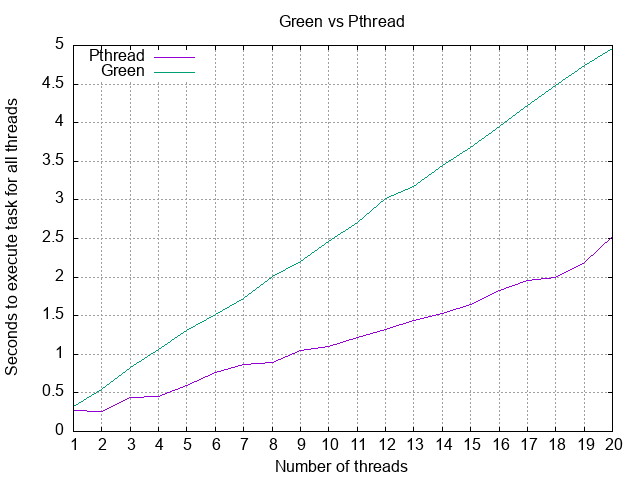
\includegraphics[width=11.2cm]{green_vs_pthread.png}
    \caption{A comparison between our green library and pthread library}
    \label{fig:graph}
\end{figure}

\noindent As visible in figure 1 the green threads take much longer than the pthreads library to execute the same benchmark despite operating in user space which should theoretically be faster than kernel space. However this is not that shocking as the pthread library is far more optimized in may more ways than the green functions that are implemented. It could also be that the operating systems scheduler treats separate threads better than a single process that contain multiple threads and hence the single process will be less favored and be scheduled less compared to the chance of one of multiple threads being scheduled. However, in the end it is most likely due to the quality of implementation of either library that makes the difference.
\newpage
\subsection*{Context switching}
Switching context is another drawback of a threaded compared to a non-threaded workload. Every time the context is loaded in and out of the heap it takes a few CPU cycles to set everything up for the next thread. This impact can be measure by introducing a yield call after line 21 in the benchmark code. This will cause the next thread to be scheduled prematurely after a number has been checked for primality rather than after each timer interrupt.

\begin{figure}[htp]
    \centering
    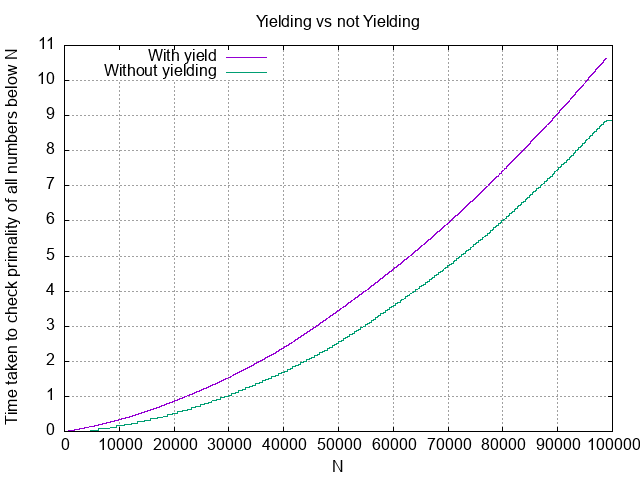
\includegraphics[width=11.2cm]{yield_vs_noyield.png}
    \caption{A comparison between yielding and not yielding}
    \label{fig:graph}
\end{figure}

\noindent In figure 2 the conclusion that yielding and inducing more context switching does have a measurable impact on the performance of the benchmark. It is of course not ideal if up to 20\% of the time taken to run a program is used for context switching. This is something the end user needs to be aware of when they are using a threading library and make sure to use the minimum number of threads needed.

\section*{Conclusion}
The new implementation of the green threading library was vastly outperformed by the built-in pthreads library. This is almost expected since pthreads has been far more optimized and was not created on a Monday afternoon. However overall the implementation of green threads has been a fun great learning experience, despite the difficult debugging, unpredictable behaviour, and the overexpose to segmentation faults. Some further exploration could be done into the use of different scheduling strategies as currently the linear first in first out ready-queue is very one dimensional and assumes that each thread has equal priority, which in the real world is not the case. 

\end{document}
